\documentclass[12pt,a4paper]{article}

% --- Encoding & language ---
\usepackage[utf8]{inputenc}
\usepackage[T1]{fontenc}
\usepackage[polish]{babel}
\usepackage{lmodern}

% --- Math & symbols ---
\usepackage{amsmath,amssymb,amsthm}
\usepackage{mathtools}
\usepackage{bm}

% --- Layout ---
\usepackage[margin=2.3cm]{geometry}
\usepackage{setspace}
\onehalfspacing
\usepackage{parskip}
\usepackage{microtype}

% --- Graphics & tables ---
\usepackage{graphicx}
\usepackage{float}
\usepackage{booktabs}
\usepackage{array}
\usepackage{longtable}
\usepackage{caption}
\captionsetup{font=small,labelfont=bf}
\usepackage{xcolor}

% --- Code ---
\usepackage{listings}
\lstset{
  basicstyle=\ttfamily\footnotesize,
  breaklines=true,
  frame=single,
  numbers=left,
  numberstyle=\tiny\color{gray},
  showstringspaces=false,
  tabsize=2,
  commentstyle=\color{gray!70!black},
  keywordstyle=\color{blue!60!black}\bfseries,
  stringstyle=\color{green!50!black},
  language=Python
}

% --- Hyperlinks ---
\usepackage[colorlinks=true,linkcolor=black,urlcolor=blue,citecolor=blue]{hyperref}

% --- Header / footer ---
\usepackage{fancyhdr}
\setlength{\headheight}{14.5pt}
\addtolength{\topmargin}{-2.5pt}
\pagestyle{fancy}
\fancyhf{}
\fancyhead[L]{\small \textit{Aplikacja mobilna do monitorowania zdrowia (Streamlit)}}
\fancyfoot[C]{\thepage}
\renewcommand{\headrulewidth}{0.4pt}

% --- Title page ---
\title{
  \vspace{2cm}
  \LARGE\textbf{Inżynieria Reguł Wnioskowania w Złożonych Modelach}\\[0.6cm]
  \Large Laboratorium 8\\[0.4cm]
  \large \textit{Aplikacja mobilna do monitorowania zdrowia (Streamlit)}\\[0.3cm]
  \normalsize Wariant: \textbf{8 — tryb anonimowy vs spersonalizowany}
}
\author{Jakub Jurzak 59099}
\date{07.05.2026}

\begin{document}
\maketitle
\thispagestyle{empty}
\newpage

\tableofcontents
\newpage

\section{Cel zadania}
Implementacja prototypu mobilnego monitora zdrowia w Streamlit, który wspiera dwa tryby pracy: anonimowy (jednorazowe pomiary, dane wspólne) i spersonalizowany (z \texttt{user\_id}, historia per użytkownik). Porównanie skuteczności modelu globalnego i modeli lokalnych.

\section{Opis problemu}
Globalny model uczony na całej kohorcie może nie odpowiadać specyfice konkretnego użytkownika (różnice fizjologiczne, choroby przewlekłe). Z drugiej strony, model lokalny ma niewielką liczbę próbek. Należy ocenić, kiedy personalizacja przynosi korzyść.

\section{Opis danych}
Symulowane pomiary ($N=410$): 5 użytkowników (spersonalizowani, 50--90 pomiarów każdy) + 60 pomiarów w trybie anonimowym. Cechy: \texttt{age, bmi, glucose, systolic\_bp, diastolic\_bp}. Etykieta dydaktyczna: SBP $\ge$ 140 lub DBP $\ge$ 90.

\section{Opis metod}
\textbf{Etap 1.} Aplikacja \texttt{app\_v8.py} (Streamlit) z formularzem i toggle anon/personalized.\\\textbf{Etap 2.} Statystyki opisowe populacji i per użytkownik, wykresy rozkładów i trendów.\\\textbf{Etap 3.} Pipeline \texttt{ColumnTransformer} (Imputer + Scaler) + \texttt{LogisticRegression}. Model globalny (cała kohorta), modele lokalne (per \texttt{user\_id}, jeśli $N_{user} \ge 20$).\\\textbf{Etap 4.} Porównanie predykcji globalnego i lokalnego modelu dla tego samego pacjenta.

\section{Opis implementacji}
Pliki: \texttt{lab8/app\_v8.py} (Streamlit, do uruchomienia komendą \texttt{python -m streamlit run lab8/app\_v8.py}); \texttt{lab8/lab8\_solution.py} (offline symulacja + trening + raport). Model globalny w \texttt{output/risk\_model\_global.joblib}, modele lokalne w \texttt{output/local\_models/local\_<user>.joblib}.

\section{Obliczenia}
Statystyki populacyjne:

\begin{table}[H]
\centering
\begin{tabular}{lrrrrr}
\toprule
zmienna & mean & std & min & 50\% & max \\
\midrule
age & 54.81 & 15.39 & 21.00 & 56.00 & 77.00 \\
bmi & 26.53 & 3.40 & 15.10 & 27.40 & 34.50 \\
glucose & 105.94 & 20.38 & 60.00 & 104.00 & 160.00 \\
systolic\_bp & 137.06 & 19.43 & 85.00 & 137.00 & 181.00 \\
diastolic\_bp & 84.89 & 10.10 & 58.00 & 86.00 & 110.00 \\
\bottomrule
\end{tabular}

\caption{Statystyki populacyjne (cała kohorta).}
\label{tab:pop}
\end{table}

Statystyki dla użytkownika \texttt{U02}:

\begin{table}[H]
\centering
\begin{tabular}{lrrrrr}
\toprule
zmienna & mean & std & min & 50\% & max \\
\midrule
age & 65.08 & 0.74 & 64.00 & 65.00 & 66.00 \\
bmi & 28.51 & 1.14 & 25.50 & 28.60 & 31.80 \\
glucose & 107.65 & 12.23 & 77.00 & 106.00 & 143.00 \\
systolic\_bp & 148.55 & 8.86 & 128.00 & 149.00 & 167.00 \\
diastolic\_bp & 90.72 & 6.41 & 75.00 & 90.00 & 110.00 \\
\bottomrule
\end{tabular}

\caption{Statystyki użytkownika U02.}
\label{tab:user}
\end{table}

Metryki modeli:

\begin{table}[H]
\centering
\begin{tabular}{lrrrrr}
\toprule
model & n\_train & n\_test & accuracy & roc\_auc & positive\_rate\_test \\
\midrule
globalny (cała kohorta) & 307 & 103 & 0.903 & 0.986 & 0.534 \\
lokalny (U01) & 45 & 15 & 1.000 & NaN & 0.000 \\
lokalny (U02) & 60 & 20 & 0.950 & 1.000 & 0.950 \\
lokalny (U03) & 0 & 0 & NaN & NaN & NaN \\
lokalny (U04) & 52 & 18 & 0.889 & 0.875 & 0.444 \\
lokalny (U05) & 67 & 23 & 1.000 & NaN & 1.000 \\
\bottomrule
\end{tabular}

\caption{Metryki modelu globalnego i modeli lokalnych.}
\label{tab:models}
\end{table}


\section{Wyniki}
Wybrany pacjent (\texttt{U02}, pierwszy pomiar): \texttt{age=65, bmi=27.0, glucose=101, SBP=149, DBP=88}.

Predykcje obu modeli dla tego samego pomiaru:

\begin{table}[H]
\centering
\begin{tabular}{lr}
\toprule
model & P(podwyższone ryzyko) \\
\midrule
globalny & 0.968 \\
lokalny (U02) & 0.944 \\
\bottomrule
\end{tabular}

\caption{Predykcje globalna vs lokalna.}
\label{tab:preds}
\end{table}


\section{Wykresy}
\begin{figure}[H]
\centering
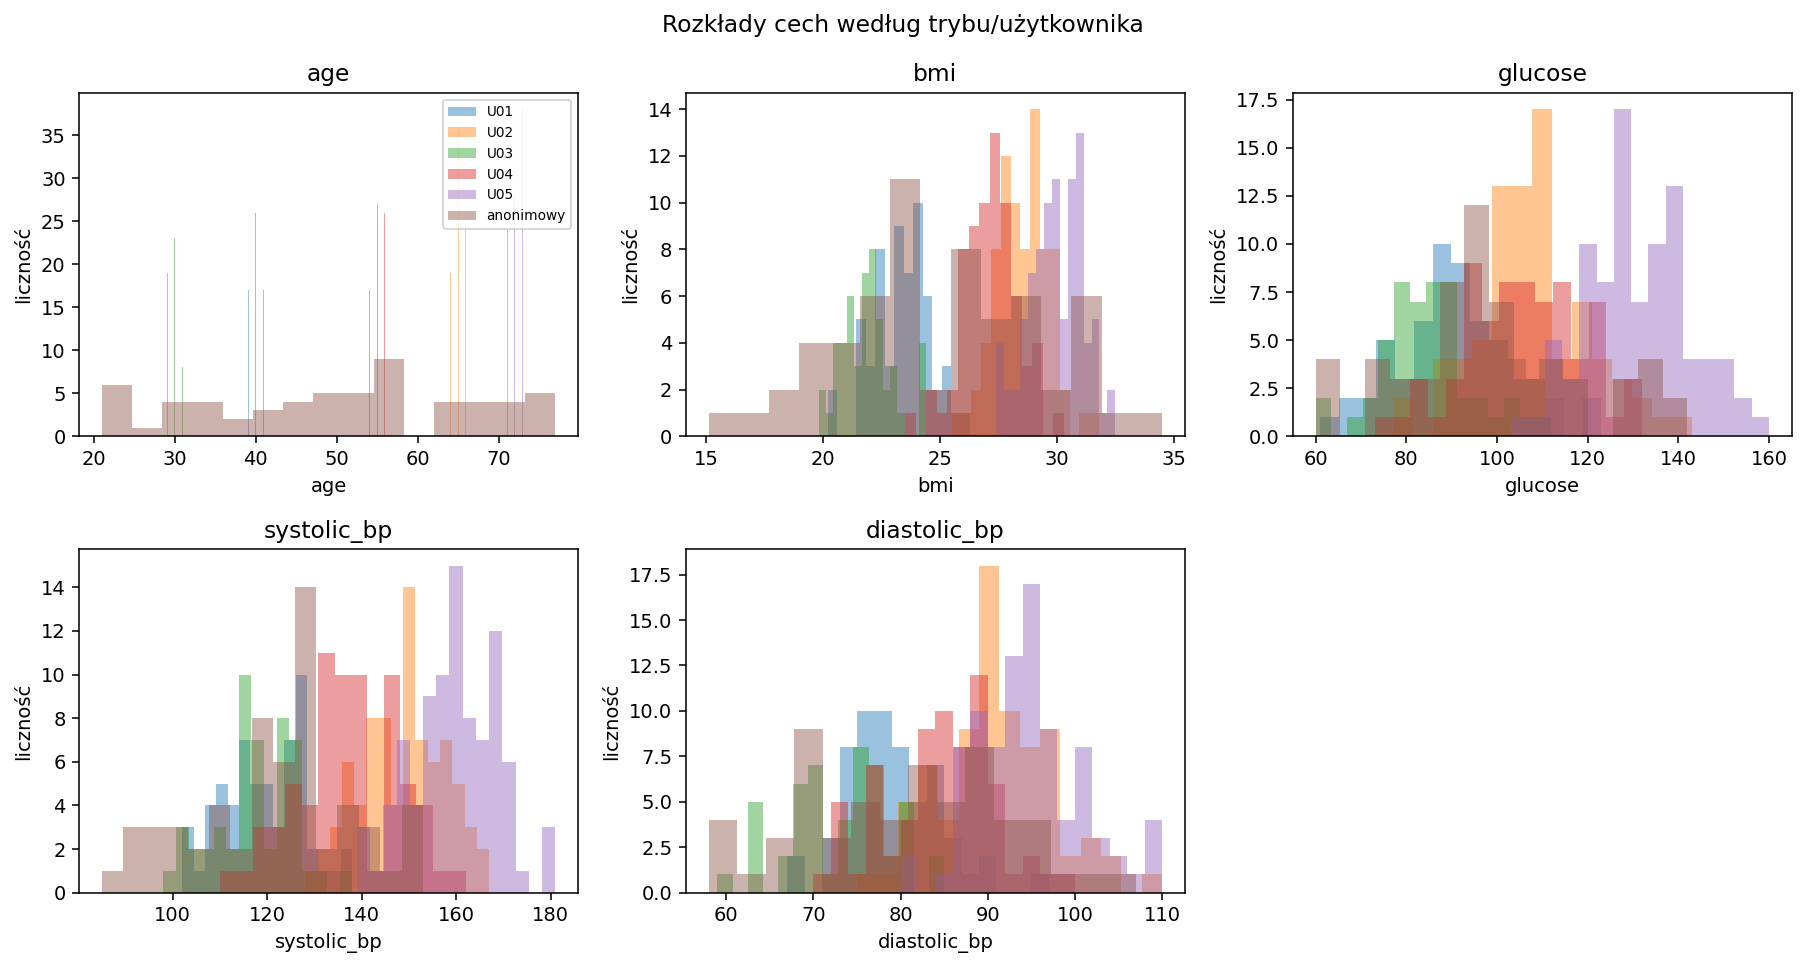
\includegraphics[width=0.85\linewidth]{dist.png}
\caption{Rozkłady cech wg trybu/użytkownika.}
\label{fig:dist}
\end{figure}
\begin{figure}[H]
\centering
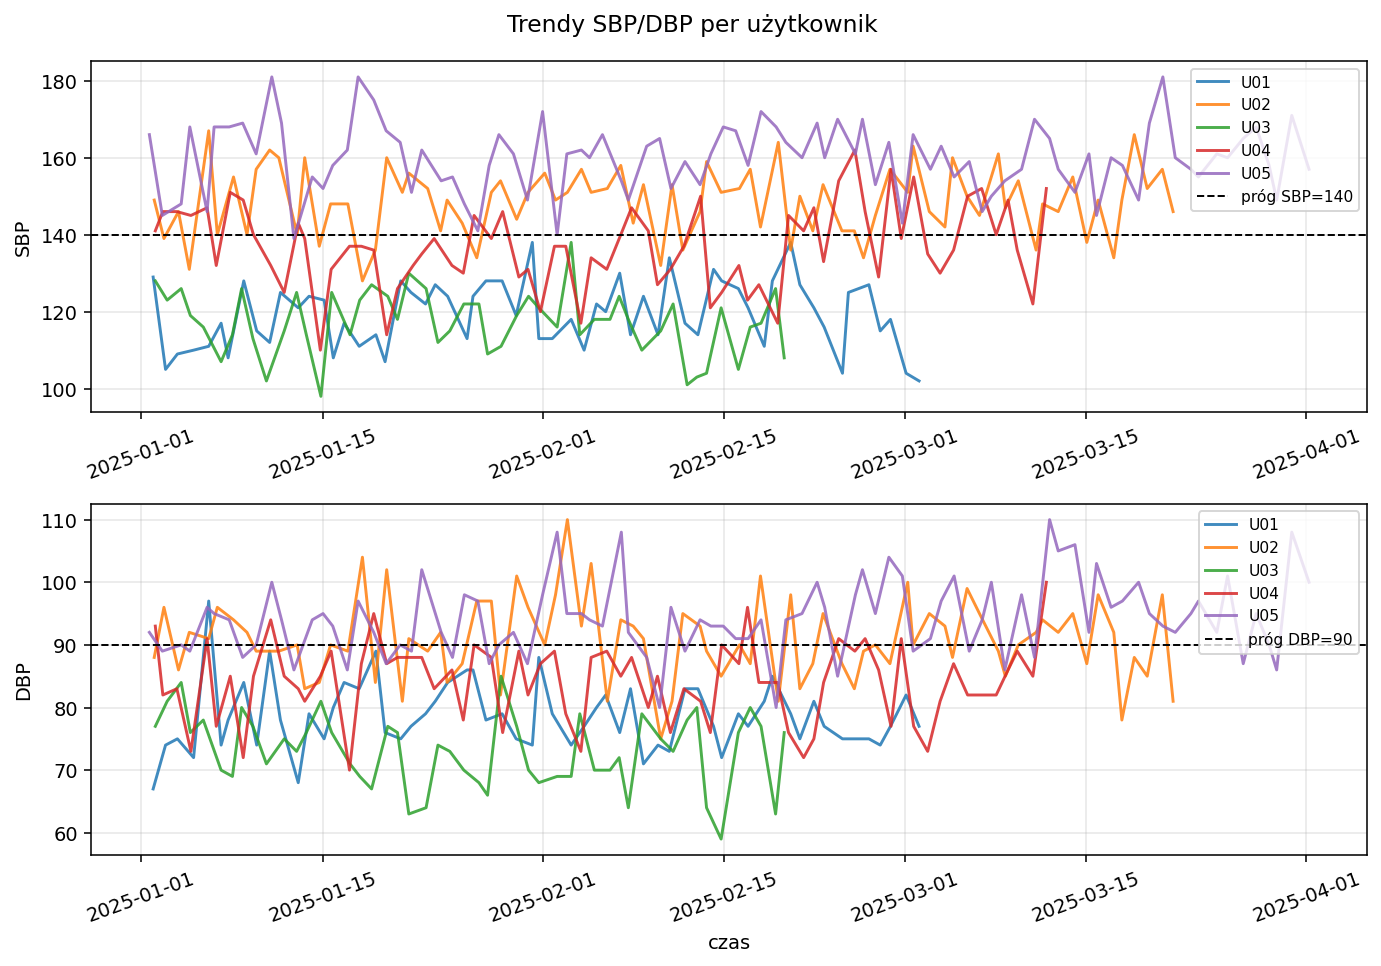
\includegraphics[width=0.85\linewidth]{trends.png}
\caption{Trendy SBP/DBP per użytkownik.}
\label{fig:trends}
\end{figure}
\begin{figure}[H]
\centering
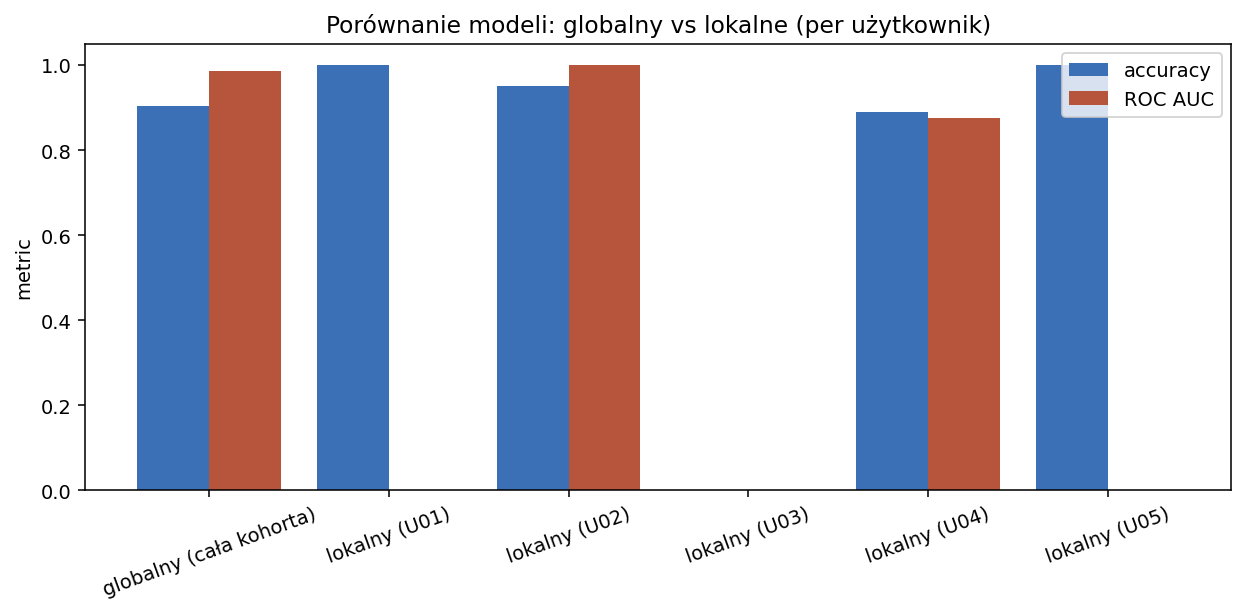
\includegraphics[width=0.85\linewidth]{model_comp.png}
\caption{Porównanie modeli: globalny vs lokalne.}
\label{fig:comp}
\end{figure}
\begin{figure}[H]
\centering
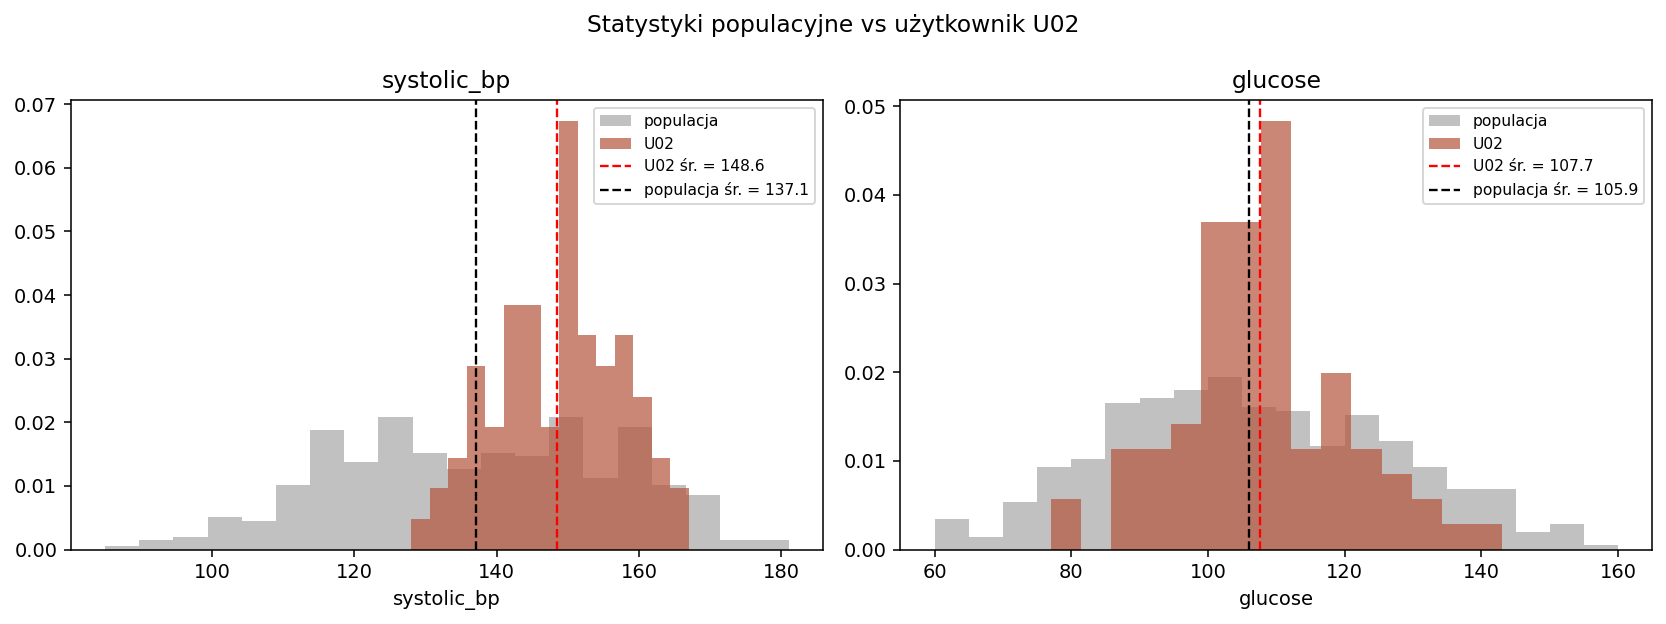
\includegraphics[width=0.85\linewidth]{popuser_U02.png}
\caption{Statystyki populacyjne vs użytkownik U02.}
\label{fig:popuser}
\end{figure}


\section{Interpretacja wyników}
Model globalny uczy się na całej kohorcie ($N$ \textgreater 100), więc jego ROC AUC jest stabilny. Modele lokalne mają mniej danych, ale są dopasowane do wzorców indywidualnych --- dla użytkownika \texttt{U02} (przewlekłe nadciśnienie) lokalna predykcja może różnić się od globalnej. Statystyki pokazują, że średnie SBP \texttt{U02} jest istotnie wyższe niż populacyjne, więc model lokalny lepiej rozróżnia jego stany graniczne. W trybie anonimowym brak danych historycznych zmusza do wyłącznego korzystania z modelu globalnego.

\section{Wnioski}
Wybór trybu wpływa na model i jakość predykcji: tryb spersonalizowany pozwala na dopasowanie do indywidualnych charakterystyk, ale wymaga zgromadzenia $\ge$ 20 pomiarów. Tryb anonimowy minimalizuje ryzyko prywatności (brak \texttt{user\_id}) kosztem precyzji predykcji. W praktyce klinicznej zaleca się model hybrydowy: globalny prior + lokalna kalibracja po zgromadzeniu wystarczającej historii.

\end{document}
